\chapter[Introduction]{\thechapter. Introduction}
\section{Intention of project}
The scope of this project is aimed to help understand and identify the advantages and/or disadvantages of the diverse modeling languages. \newline
Using different graphical models provided by a certain modeling language, one is able to make a precise specification of a complex system. Based on this specification and the fact that the process of modeling is abstract from the process of implementing, is the probability for misunderstandings, due to insufficient communication, very low.\newline
In order to ensure meaningful assessment of the diverse modeling languages, a standardized software architecture need to be modeled, like the one offered by Automotive Open System Architecture (AUTOSAR). Because of the broad scope and variety of software layers presented in AUTOSAR architecture as show in Figure 1.1, only the memory stack is going to be modeled.  The main reason for this decision is that the memory stack is to be found in every automotive unit\footnote{Leitner Fl. $\-$ Evaluation of the Matlab Simulink Design Veri�er versus the model checker, S. 24}.
\begin{center}
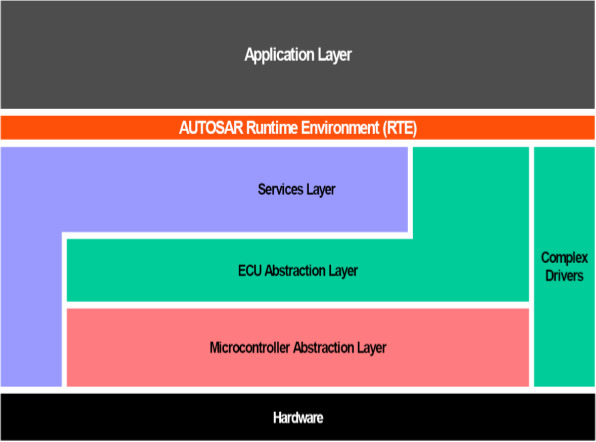
\includegraphics[scale=0.45]{Images/Figure1_1.png}\\
Figure 1.1 - AUTOSAR Architecture
\end{center}
\section{Goals and success criteria of project}
The project activities are going to be comparable to the base practices(BP) defined by the Software Process Improvement and Capability Determination(SPICE) model.
\begin{itemize}
\item BP1 - Software architectural design - 30.10.2009
\item BP2 - Software requirements - 06.11.2009
\item BP3 - Define interfaces - 20.11.2009
\item BP4 - Dynamic behavior - 27.11.2009
\item BP6 - Detailed design - 28.12.2009
\item BP7 - Verification criteria - 11.01.2010
\item BP8 - Verify Software design - 18.01.2010
\item BP9 - Consistency and Bilateral Traceability - 28.01.2010
\end{itemize}
The BP5 and BP10 cannot be done in this setting due to missing work products. The project is successfully completed if the results are meaningful in industrial practice.